% This is LLNCS.DEM the demonstration file of
% the LaTeX macro package from Springer-Verlag
% for Lecture Notes in Computer Science,
% version 2.4 for LaTeX2e as of 16. April 2010
%
\documentclass{llncs}
%
\usepackage{makeidx}  % allows for indexgeneration
\usepackage{booktabs}
\usepackage{todonotes}
\usepackage{microtype}
%
\begin{document}
%
\title{Learning Split and Merge Errors in Electron Microscopy Cell Segmentations to Assist Connectomics Proofreading}
%
\titlerunning{Learning Split and Merge Errors}  % abbreviated title (for running head)
%                                     also used for the TOC unless
%                                     \toctitle is used
%
\author{Daniel Haehn\inst{1,2} \and Verena Kaynig-Fittkau\inst{1,2}
\and James Tompkin\inst{1} \and Hanspeter Pfister\inst{1,2}}
%
\authorrunning{Daniel Haehn et al.} % abbreviated author list (for running head)
%
%%%% list of authors for the TOC (use if author list has to be modified)
\tocauthor{Daniel Haehn, Verena Kaynig-Fittkau, James Tompkin, and Hanspeter Pfister}
%
\institute{Harvard Paulson School of Engineering and Applied Science, and\\
\and
Harvard Center for Brain Science, Cambridge MA 02138, USA}

\maketitle              % typeset the title of the contribution

\begin{abstract}
Automatic image segmentation methods for cells can lead to \emph{split errors}, where one cell is accidentally labeled as two or more, and to \emph{merge errors}, where two or more cells are accidentally labeled as one. We develop two classifiers which, given an input image and a candidate set of cell labelings, are able to identify split and merge errors in the segmentation. These classifiers are informed by supervised training of a convolutional neural network: from expert-labelled ground truth segmentations, and their corresponding input images and edge probabilities, we synthetically generate plausible split and merge errors as training. We design a new network architecture which is able to determine a true edge with high accuracy by considering a  wider uncertainty region around an edge as an additional input to the network. We demonstrate the application of this approach to proofreading of electron microsopy image segmentations for connectomics, where our system is able to automatically correct many errors, and otherwise prioritize a list of edges to which a human should direct their attention for manual correction.
\keywords{Segmentation, convolutional neural networks, connectomics.}
\end{abstract}
%

\section{Introduction}

% JT: Trying to write short, as we have only 8 pages.
%\JT{EVERYONE: I am a bit concerned about two reductionist arguments that will be thrown at us: 1. why don't we just try and make the initial segmentation better? 2. at the limit, someone still has to scan the whole volume because your edge error classifier is often wrong. Any ideas?}

%Paragraph one: Provide context to the work.
%What is the task? What is the state of the task?
In connectomics, neuroanatomists build 3D reconstructions of neuron connectivity to gain insight into the functional structure of the brain. Rapid progress in automatic sample preparation and electron microscopy (EM) acquisition techniques has made it possible to image volumes of brain tissue at $\approx6nm$ per pixel to identify synapses and vesicles. For a section $25nm$ thick, a $1 mm^3$ volume of brain tissue contains $10^{15}$ voxels, or 1 petabyte of data. Manual annotation of data this large is unfeasible, and automatic methods are needed \cite{jain2010,kaynig13,Liu2014,NunezIglesias2013Machine,GALA2014,amelio_segmentation}.

Automatic segmentation and classification of brain tissue is hard in cases with ambiguous intercellular space \cite{isbi_challenge}, so learning-based methods are common. These can be based on interactive learning with random forests \cite{neuroproof2013,amelio_segmentation,kaynig13}, or supervised learning with convolutional neural networks \cite{RonnebergerFB15,lee2015recursive}, or potentially even with unsupervised learning \cite{BogovicHJ13}. Typically, cell membranes are learned in 2D images and then grouped into geometrically-consistent cell regions across registered sections to form 3D volumes, or learned across registered sections in 3D directly. Using dynamic programming techniques \VKF{cite cdd whole image training paper}, and small GPU clusters, these classifiers can segment about 1 terabyte of data per hour \cite{kasthuri2015saturated}, and so `keep up' with the data capture process on state-of-the-art electron microscopes.

%State of the art methods use convolutional neural networks to learn cell membranes in 2D images from hand-labeled training data. Then, labeled membranes are grouped into geometrically-consistent cell regions across sections to form 3D image stacks. Using dynamic programming techniques \VKF{cite cdd whole image training paper}, and small GPU clusters \VKF{how many?}, these classifiers can segment about 1 terabyte of data per hour \cite{kasthuri2015saturated,lee2015recursive}, which is the rate necessary to keep up with the data capture process on state-of-the-art electron microscopes. %\VKF{citation for 61 beam microscope?}. \JT{I would skip. There is a Nature press piece (see comment in source), but is there a peer-reviewed academic article? Also, I cited the recent Cell paper for the segmentation rates above; I hope that is ok.} % \url{http://www.nature.com/nature/journal/v503/n7474/full/503147a.html?WT.ec_id=NATURE-20131107}

%Paragraph two: What is the problem in this context? What is the situation that you are trying to correct or overcome?
However, all automatic methods are at least somewhat erroneous, and we are left with large volumes of data which need \emph{proofreading}. This crucial task serves two purposes: 1) to correct errors in the segmentation for later use, and critically 2) to provide larger corpora of labeled data to train better automatic segmentation methods. Recent interactive proofreading tools provide intuitive user interfaces to browse segmentation data in 2D and 3D and identify and manually correct errors \cite{markus_proofreading,raveler,mojo2,haehn_dojo_2014}. Many kinds of errors exist, such as inaccurate boundaries, but the most egregious are \emph{split errors}, where a single cell is labeled as two, and \emph{merge errors}, where two cells are labeled as one. With user interaction, split errors can be joined, and the missing edge in merge errors can be discovered with techniques like manually-seeded watersheds \cite{haehn_dojo_2014}. However, even with these `semi-automatic' correction tools, the visual inspection of the data to find the errors in the first place takes the majority of the time.

%Paragraph three: What is the proposed solution at a high level? What is the result of the method, and how does it impact the problem?
Our goal is to complement semi-automatic correction tools with semi-automatic error finding. Instead of having to visually inspect the whole data volume carefully to spot any errors, we design two automatic classifiers which detect both split and merge errors in 2D segmentations, to direct the user to regions with a high probability of an error. Then, we suggest probable error corrections for the user to accept or reject. Given an initial membrane segmentation from an automatic method, our classifiers operate on whole cell regions. This significantly reduces the data volume and allows us to employ large convolutional neural networks which take a greater region of context and multiple input channels into account.

One major reason for attempting to classify errors on 2D images is with the scale of the task. 3D reconstruction pipelines are often slow as they require non-linear image alignment or registration \cite{akselrod09,beyer13,Saalfeld2010Asrigidaspossible}. However, typically segmentation results are local decisions at the cell level. In this case, reconstruction is unnecessary and, instead of waiting for the 3D output, proofreading can start immediately to maximize throughput.

%Paragraph five: Optimistically, what is the consequence of the method - what can I do now that I could not do before?
We validate our approach in a purely automatic mode, and in an experiment against an existing proofreading tool with only semi-automatic merge error correction\cite{haehn_dojo_2014}. We discover that our automatic corrections reduces variation of information (VI) vs.~ground truth expert segmentations from 0.59 to 0.49, and that, with users, our automatic error suggestions and corrections can potentially decrease VI from 0.56 to 0.48. As a consequence, we are able to provide tools to proofread segmentations more efficiently, from which to improve automatic segmentation methods and better tackle vast volumes of connectomics imagery.

%\subsection{Contributions}
%
%Given this, we contribute to the literature:
%\begin{enumerate}
%\item One contribution
%\item Two contribution
%\item (Maybe) three contribution
%\end{enumerate}
%
%\begin{figure}
%\missingfigure{Example of a fixed split error. Example of a fixed merge error.}
%\caption{Example of a fixed split error. Example of a fixed merge error.}
%\end{figure}
\section{Related Work}

Paragraph: Work on segmentation in Connectomics...but none of these address specifically learning real edges against edges which lead to split or merge errors.

Arganda-Carreras et al.~\cite{10.3389/fnana.2015.00142} posed the ISBI 2D EM segmentation challenge in 2012, where a 30-image corpus of fly cell `in/out' labels was used to train boundary detection. To overcome the often small amounts of expert-labeled ground-truth segmentation data for training convolutional networks for biomedical tasks, Ronneberger et al.~\cite{RonnebergerFB15} use a contracting/expanding path architecture to enable precise localization.

The data we are most concerned with is more difficult than the ISBI 2012 challenge. Our mouse brain data has large intercellular space which is not b

Paragraph: Work on learning in Connectomics

Paragraph: Most related work. People tried this for 3D! \cite{BogovicHJ13}. 

\paragraph{Interactive segmentation}

Recent works attack the problem of massive volume segmentation through crowd-sourcing\cite{saalfeld09,anderson2011}. EyeWire~\cite{eyewire2012} asks novice users to participate in a segmentation game for segmenting neuronal structures using a semi-automatic algorithm. D2P ~\cite{Giuly2013DP2} uses a micro-labor workforce approach where local boolean decisions are combined to produce a consensus segmentation. NeuroProof \cite{neuroproof2013} allows interactive learning of agglomeration of over-segmentations of images, based on a random forest classifier. In general, our goal is to correct the output of a segmentation which is thought to be good; hence, our tool would be used after learning a segmentation model to direct user attention to correct likely erroneous areas.

\paragraph{Proofreading Tools}
Recent works in segmentation proofreading have begun to move towards semi-automatic methods. Raveler~\cite{raveler} targets expert users and offers many parameters for tweaking the process at the cost of a higher complexity. Sicat et al.~\cite{markus_proofreading} propose guiding the user to problem areas through a graph abstraction of potential problematic regions. Mojo~\cite{mojo2} and its follow-up Dojo~\cite{haehn_dojo_2014} provide semi-automatic merge error correction, though manual error finding is still required.


Why don't we do 3D? Mega pipeline - people need to start proof-reading as soon as possible, need to maximize throughput. If we can do a good job on 2D, it eases this process as we can start working before the alignment stages.

\subsection{Contributions}

Given this, we contribute to the literature:
\begin{enumerate}
\item One contribution
\item Two contribution
\item (Maybe) three contribution
\end{enumerate}
\section{Method}
%Paragraph one: Overview of the method. What are the high level steps taken to build the system? What are the key techniques used within the system?
We identify split errors in the segmentation using a convolutional neural network (CNN). The network is designed to scan existing boundaries in the segmentation and provide a score on how likely this edge causes a split error. We use this trained CNN in the detection and correction of split errors as well as merge errors as follows.

For split errors we classify existing boundaries in the segmentation according to if they cause a split error or not. Detecting a split error boundary automatically allows to correct the split error as removing the detected edge corrects the error and merges the two split regions into one correct segment. 

Identification and correction of merge errors is challenging, because the correction of a merge error requires the generation of a new edge in the segmentation, which was missed by the automatic segmentation before. To address this problem we generate a number \VKF{How many ?} of potential boundary candidates. If the segmented region is already correct, all of these generated boundaries should be highly ranked as split errors. If the region contains a merge error, a candidate edge that would correct this merge error would not be identified as a split error. By finding this candidate edge we identify a region as containing a merge error and obtain a boundary that can added to the segmentation to correct the error. \VKF{I think this still sounds confusing.}

\subsection{Labelled Data - Generating fake splits and merges}
\VKF{Is it true that we not generate any fake splits anymore for training? I would really like to avoid having to explain the boundary split errors we discussed in the last meeting.}

Paragraph: What is the goal of generating labeled data? How do you generate fake splits? How do you generate fake merges? How do you generate patches for training? How can we know that the training data is representative of real data?

\begin{figure}
\missingfigure{Input to learning}
\caption{Show visually each of the inputs to the system on a couple of patches.}
\end{figure}

Using only one binary mask allows us to look at merge errors over more than two regions.


\subsection{Network Design}
%Paragraph: What is the rationale behind our network design? Why do we think this will work over other approaches? 
We train a CNN to detect split errors in the segmentation. In contrast to the standard CNNs, which are the state of the art for membrane detection and automatic segmentation of electron microscopy images of brain tissue, the network trained to detect split errors takes a wider context window and multiple input channels into account. The input channels correspond to different outputs of the automatic segmentation like the boundary probability map and binary masks corresponding to segmented regions and region overlaps. The network can then leverage these multiple input patches to identify and correct errors made by the previous membrane detection network and the automatic segmentation pipeline. 

%Paragraph: What are the inputs to the design? What is the design? Parameters of the design.
The design of the network follows the design of Viren et al. \VKF{Cite Viren}, who designed a network for agglomerative clustering of oversegmentations. In contrast to Jain et al, our network operates on 2D patches instead of 3D volumes. Operating in 2D gives the advantage that we do not require images to be pre-aligned. In addition it enables a wider context window without adding too much computational complexity. \VFK{This is pretty crappy but I have trouble finding a better argumentation}

The input to the network consists of several input patches. The original design of Jain et al. included a patch from the electron microscopy image, a membrane probability map generated for the initial automatic segmentation, and a binary mask of the two regions of the potential split error. Our modified design also includes \VKF{add our inputs here}. 
Each of the input patches is connected to a \VKF{3?}-layer network, with each layer consisting of a convolutional and a pooling layer. The output of all these networks is then combined by a fully connected MLP with one hidden layer and a two class logistic regression output layer. 

Jain et al. also developed two pooling techniques employed in the pooling layers of the CNN, dynamic boundary pooling and dynamic object pooling. The idea is to focus the pooling output on regions of interest, like the boundary between two regions (boundary pooling), or the joint area of the two regions considered (object pooling). Instead of convential pooling where a sliding window is equally applied to the whole output of the convolutional layer, dynamic pooling only averages outputs within the region of interest. We implemented both pooling methods and compare them in table \VKF{reference to result table}.

\begin{figure}[t]
\missingfigure{Network architecture figure}
\caption{Network architecture diagram, showing parallel sub nets that feed into a multi-layer perceptron at the end.}
\end{figure}

\subsection{Training}

Paragraph: How did we train the network? What tricks did we employ (e.g., rotation)? What are the parameters of the training? What software stack did we use? Hardware platform, training time (none very interesting, but for completeness). When do we stop training?



Paragraph: What are the thresholds in the system? How do we pick the thresholds?


\begin{table}
\begin{tabular}{ll}
\toprule
Parameter & Value \\
\midrule
one & \\
two & \\
three & \\
\bottomrule
\end{tabular}
\caption{This is a table of parameters. This is not very interesting, but it's easier to read than in the body text and putting everything together helps the reader quickly assess.}
\end{table}
\section{Evaluation}

We evaluate our split and merge error detection and correction recommendation in the context of interactive proofreading tools: to direct users to regions with a high probability of error and to suggest corrections (Fig.~\ref{fig:results}). For comparison, we take publicly available mouse cortex data of the same kind as our training data. This data is part of the ISBI 2013 challenge training dataset ($1024\times1024\times100$ voxels) which was acquired using a serial section scanning electron microscope (ssSEM) with a resolution of $6\times6\times30\, nm$ per voxel. We use the available manually-labeled ground truth to score our approach using the variation of information (VI) metric, which is closely related to mutual information. VI is a measure of the distance between two clusterings, where lower VI numbers are better. Since our classifiers are trained on 2D image slices, we perform all evaluations on slices rather than 3D volumes. \JT{WHICH NETWORK}

\paragraph{Interactive proofreading.}
Recently, Haehn et al.~discussed requirements for interactive proofreading and evaluated three different tools on connectomics data in a study with naive users~\cite{haehn_dojo_2014}. This study asked users to spend 30 minutes proofreading with the different tools, to correct split and merge errors to improve the automatic segmentation. The best performing tool in their evaluation was Dojo. We use their findings and their user-generated proofreading result data, which they kindly provided, as a baseline for the evaluation of our method.
%The authors performed a non-expert user study and stated that their software Dojo provides better results than other tools due to a minimalistic user interface and sophisticated 3D volume rendering.
%Haehn et al. perform their user study on the most representative sub-volume ($400\times400\times10$ voxels) in terms of distribution of object size. For optimal comparison, we use exactly the same data.

To compare against Dojo, we simulate a user for proofreading correction. We assume that all classification has been computed ahead of time, and that the user is presented with a stream of error corrections to assess. The assessment is simulated by comparing the VI before and after each performed correction. Corrections are accepted only when VI reduces, and we test this across different user error rates (Fig.~\ref{fig:results}). In Haehn et al., the proofreading time was limited to 30 minutes, and human participants performed 59 corrections on average ($\approx30$ seconds per correction). In our scenario, users do not need to visually find errors and manually correct them, and so instead we assume each correction assessment takes 15 seconds (120 assessments in 30 minutes). Split errors are likely to take less time than this; however, merge errors are harder to assess, as the user must select between the top 5 candidate boundaries. Since the performance between human participants of Haehn et al.'s user study shows large variation, we present both the best performing user (VI improvement $.0598$) and the average performance among all users (VI improvement $-0.012$) as our baseline. In the simulated case, the VI improvement in comparison to the ground truth is \VKF{update $0.11$} (Fig.~\ref{fig:results}).

\paragraph{Automatic correction.} As a comparison, we also perform automatic correction. During training, we define a probability threshold $p_t=.95$ \VKF{This is actually different than the 0.7 claimed before} for automatic split correction based on CNN probability from the test set. Then, for automatic correction, we apply both classifiers to produce lists of split and merge errors sorted by confidence. First, we correct merge errors with $\max(1-p)$, followed by split error correction using $p_t$. The total time for the correcting all \JT{\#} errors was 17 minutes (\JT{\#} merge error correction 15min, \JT{\#} split error correction 2min). The average VI improvement in comparison to the ground truth was negative\VKF{update} (Fig.~\ref{fig:results}). This is not surprising, as the problem is very challenging, and this motivates the need for human-in-the-loop proofreading tools.

%\paragraph{Random proofreading.} Given the automatic result, we decided to test a classifier with random performance in comparison to our learned CNN. For split errors, the simulated user is presented with randomly picked boundaries, which they can accept or reject. For merge errors, the simulated user is presented with 5 randomly selected boundaries from the interior of the segmented region. The significantly worse performance of this approach demonstrates that our network is informative to the user.

\begin{figure}[t]
\centering
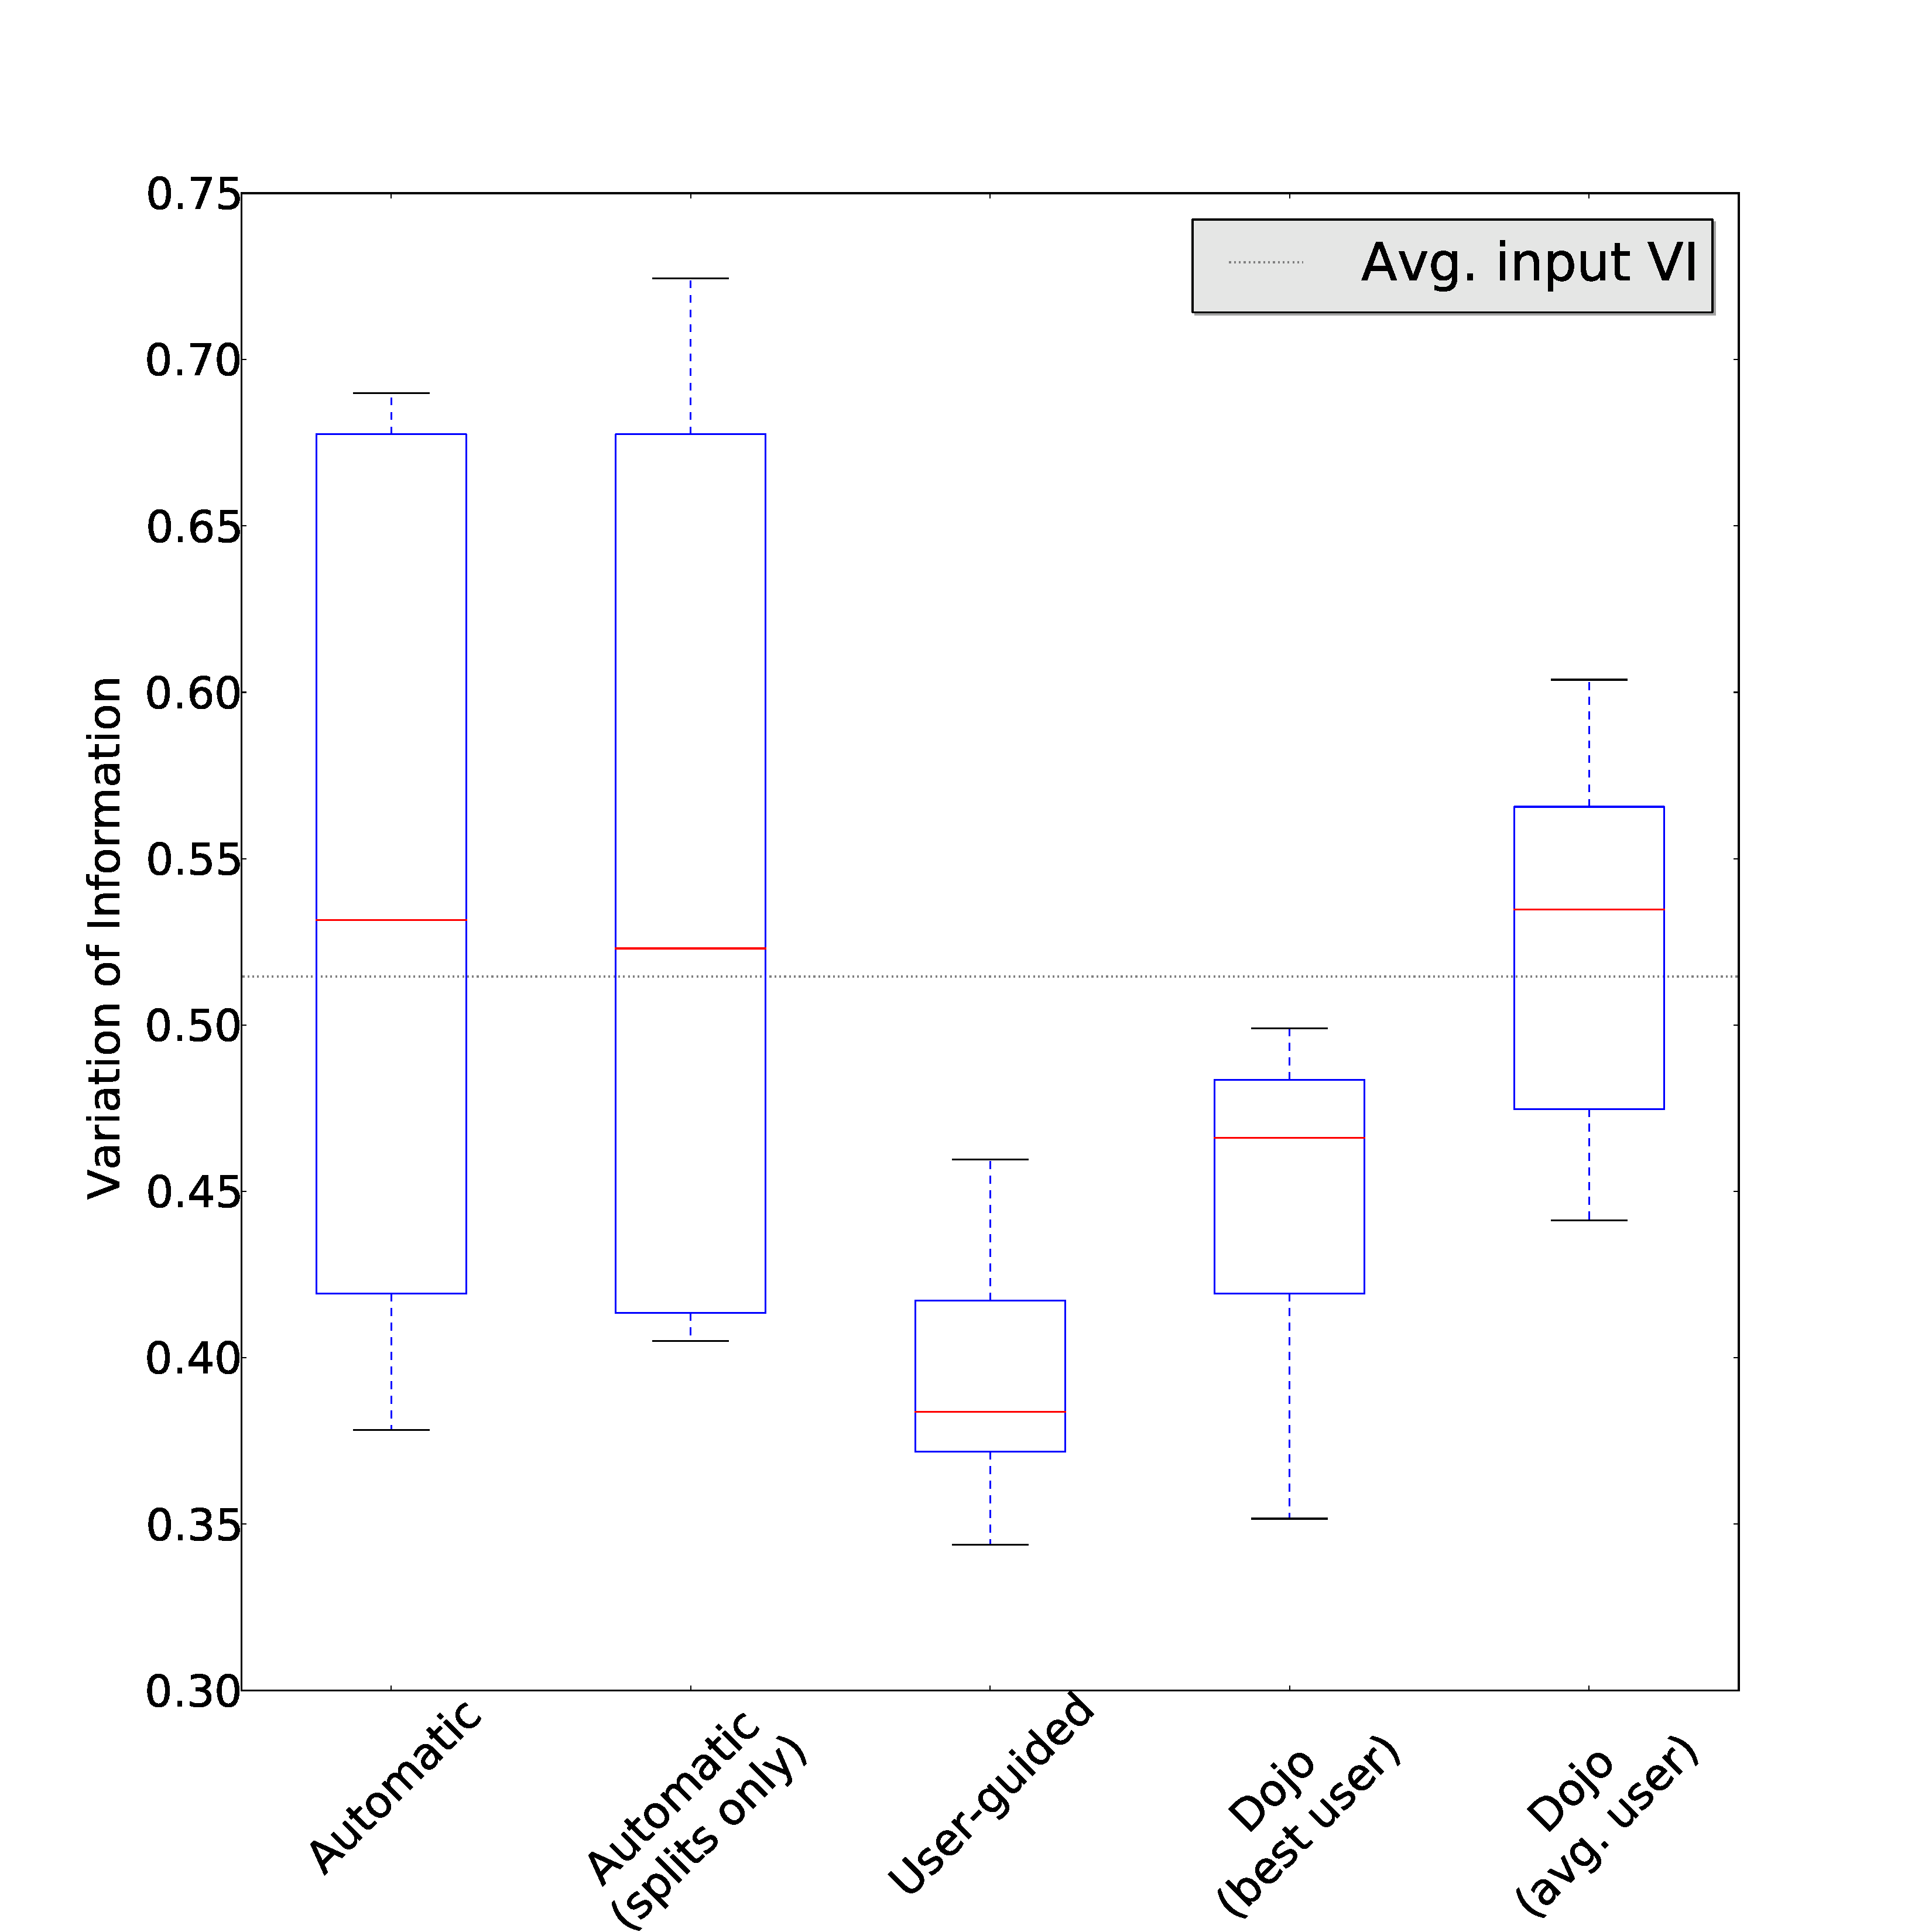
\includegraphics[scale=.15]{gfx/results_new.pdf}
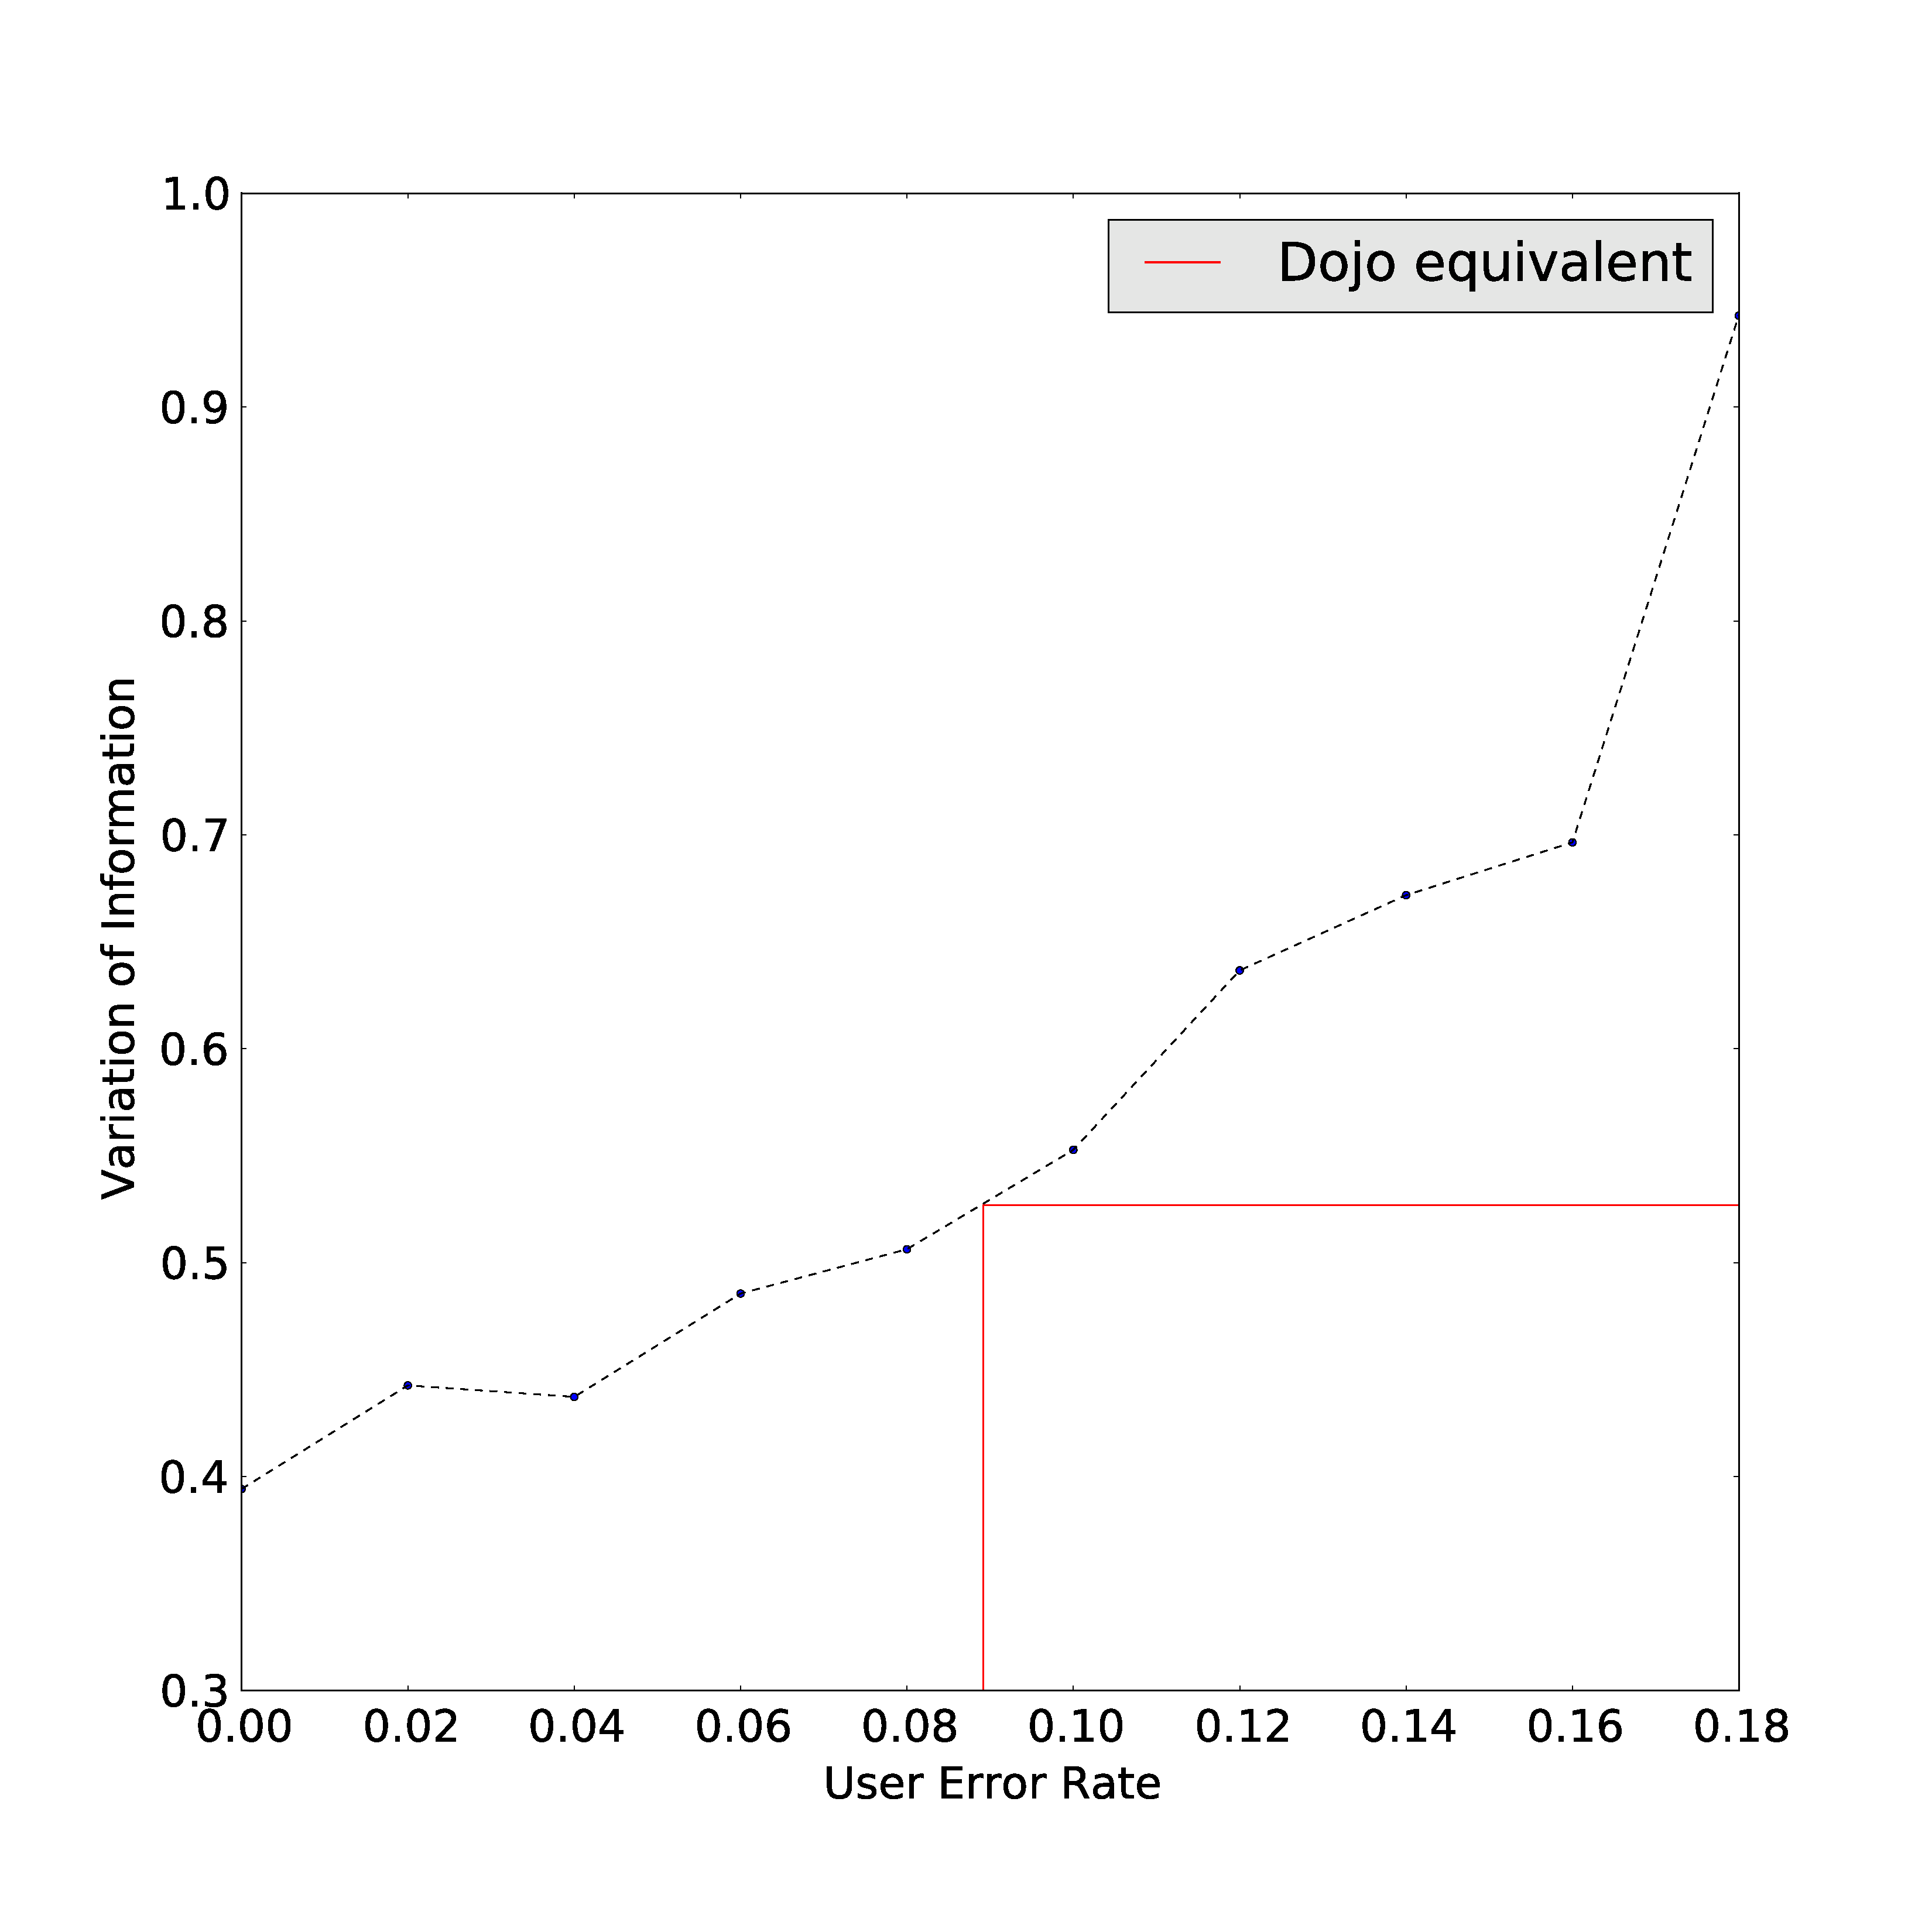
\includegraphics[scale=.15]{gfx/user_error_rate.pdf}
\caption{We compare user-guided (error rate 0.0) and automatic (full+just splits) proofreading results using our trained network,  as well as results from Haehn et al.'s comparison study \cite{haehn_dojo_2014} across 2D slices of connectomics data. The score is measured in variation of information (VI) between an input and the corresponding performance. Lower scores are better.}
\label{fig:results}
\end{figure}
%
%
%\subsection{Split error evaluation}
%
%Paragraph: What is the process of evaluating split errors?
%
%Paragraph: What do we compare against? What is the result? Why is the performance better?
%
%\begin{table}[t]
%\begin{tabular}{ll}
%\toprule
%Method & VI improvement after fixing split errors \\
%\midrule
%Jain design & \\
%Jain design variation & \\
%Our design &  \\
%Our design variation & \\
%\bottomrule
%\end{tabular}
%\caption{This is a table of results. It shows the comparison to Jain et al., and the comparison to different variations of these algorithms with the varying overlap regions.}
%\label{tab:spliterrorcorrectionperformance}
%\end{table}
%
%\subsubsection{Analysis}
%
%Paragraph: Demonstration of ROC curves for VI performance in split error adjustment as the threshold varies.
%
%\begin{figure}[t]
%\missingfigure{}
%\caption{What does the performance of split error correction look like (ROC curve) as the threshold on edge probability changes?}
%\end{figure}
%
%\subsection{Merge error evaluation}
%
%Merge errors are not that common. False positive rate is very important. Choosing threshold is important.
%
%Paragraph: What is the process of evaluating merge errors?
%
%Paragraph: What do we compare against? What is the result? Why is the performance better?
%
%\begin{table}[t]
%\begin{tabular}{ll}
%\toprule
%Method & VI improvement after fixing merge errors \\
%\midrule
%Our design &  \\
%Our design variation & \\
%\bottomrule
%\end{tabular}
%\caption{This is a table of results. It shows our ability to improve VI.}
%\end{table}
%
%
%
%Philosophical point of trading split errors for merge errors...
%
%
%Speed of classification
\section{Application}
\section{Discussion}




\section{Conclusion}

Paragraph: What we did. What the consequences of what we did are. What is now possible from what we did.

%
% ---- Bibliography ----
%
\bibliographystyle{splncs03}
\bibliography{paper_references}

\end{document}
